\documentclass[hidelinks]{ctexart}

\usepackage[singleton,margintoc]{van-de-la-sehen}

\begin{document}

\showtitle{Thomas旋进}

\begin{wrapfigure}{r}{7cm}
    \begin{tcolorbox}[sharp corners=all,boxrule=.3pt,colframe=lightgray,left=1mm, top=1mm, right=1mm, bottom=1mm]
        \CJKfamily{hwht}
        \centerline{这是\href{https://en.wikipedia.org/wiki/Spacetime}{时空}主题之一部分}\vspace{1mm}
        \centerline{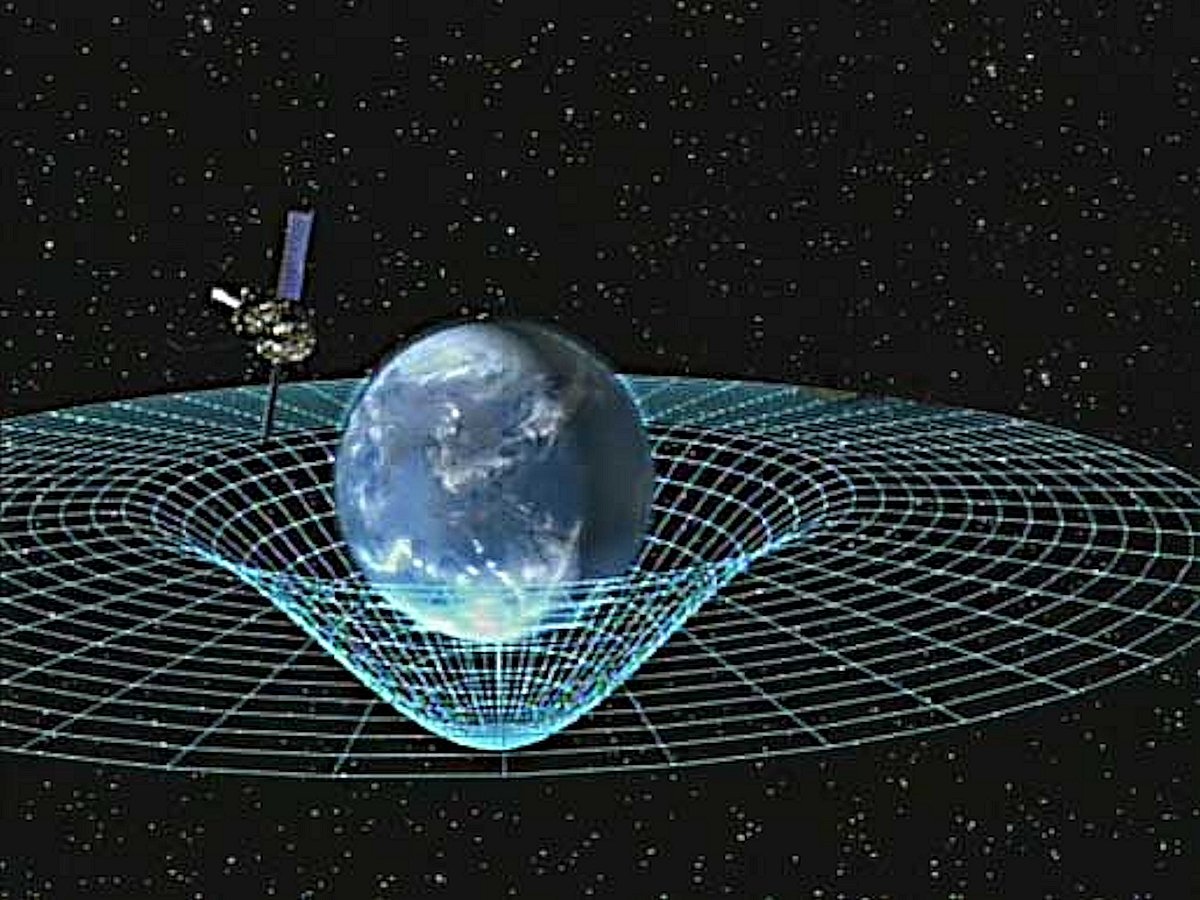
\includegraphics[width=6.5cm]{src/GPB_circling_earth.jpg}}
        %\vspace{.3em}
        \scriptsize\centerline{\href{https://en.wikipedia.org/wiki/Special_relativity}{狭义相对论}}
        %\vspace{.3em}
        \centerline{\href{https://en.wikipedia.org/wiki/General_relativity}{广义相对论}}
        \begin{tabular*}{\textwidth}{l @{\extracolsep{\fill}} r}
            时空概念 & \href{https://en.wikipedia.org/wiki/Thomas_precession}{跳转} \\
            广义相对论 & \href{https://en.wikipedia.org/wiki/Thomas_precession}{跳转} \\
            经典引力理论 & \href{https://en.wikipedia.org/wiki/Thomas_precession}{跳转} \\
            数学背景 & \href{https://en.wikipedia.org/wiki/Thomas_precession}{跳转}
        \end{tabular*}
    \end{tcolorbox}
\end{wrapfigure}
Thomas进动是对基本粒子的旋转或者宏观陀螺仪进动的相对论修正, 将角速度和曲线运动粒子的自旋联系起来.
\par
对于给定的惯性参考系, 如果有第二个参考系相对经历了Lorentz boost, 并且有第三个参考系相对第二个经历了Lorentz boost, 且第一个参考系和第三个参考系并非共线, 则第一个参考系和第三个参考系之间的变换是boost和旋转的组合, 谓Wigner旋转或Thomas旋转. 对于加速运动, 每个时刻的加速参考系都可以关联一个惯性参考系. 相隔短时间区间的两个boost可以组合成\href{https://en.wikipedia.org/wiki/Wigner_rotation}{Wigner旋转}, 对于区间无限小的极限情形加速参考系无时不刻发生旋转, 故加速参考系以一角速度旋转.
\par
\begin{wrapfigure}{r}{3.5cm}
    \begin{tcolorbox}[sharp corners=all,boxrule=.3pt,colframe=lightgray,left=1mm, top=1mm, right=1mm, bottom=1mm]
        \centerline{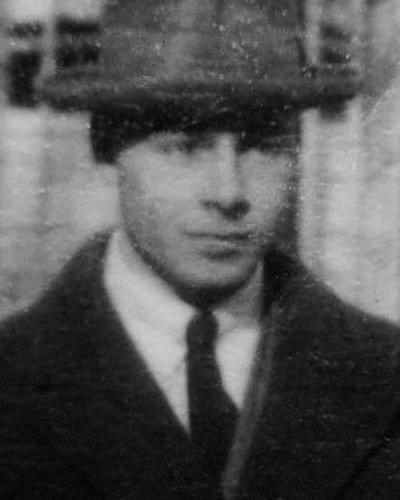
\includegraphics[width=3cm]{src/Thomas,Llewellyn_1926_Kopenhagen.jpg}}
        \scriptsize\textsf{\href{https://en.wikipedia.org/wiki/Llewellyn_Thomas}{Llewellyn Thomas} (1903 -- 1992)}
    \end{tcolorbox}
\end{wrapfigure}
这一进动可以被几何地解释为相对论中的速度空间是双曲的, 故其中绕圆(即绕着线速度)的平行移动(即平行移动角速度)导致它指向完全不同的方向, 或者代数地解释为\href{https://en.wikipedia.org/wiki/Lorentz_transformation}{Lorentz变换}的不可交换性. Thomas旋进可以正确给出自旋-轨道耦合, 这考虑了电子和原子核之间的钟慢效应.
\par
Thomas旋进是狭义相对论的平直时空的动力学效应. 对于广义相对论的弯曲时空情形, Thomas进动需要和几何效应结合得到\href{https://en.wikipedia.org/wiki/Geodetic_effect}{de Sitter效应}. 虽然Thomas效应完全是运动学效应, 只有在曲线运动中它才会出现, 因此无法在不存在外力的情形下被单独观测到, 故Thomas旋进通常会伴随动力学效应.
\par
如果系统不受外力矩, 例如在外标量场的情形, 其自旋的动力学直接由Thomas旋进决定. 一个独立的Thomas旋转(相对于一系列无限小的Thomas旋转组合成的Thomas进动)会在有多个非共线运动的惯性参考系的情形下出现, 并可由Lorentz变换导出.

\section{历史} % (fold)
\label{sec:历史}

Thomas旋进最早由\href{https://en.wikipedia.org/wiki/Ludwik_Silberstein}{Ludwik Silberstein}在1914年发现. 但是Thomas仅有的关于相对论性进动的知识来源于de Sitter关于月球的相对论性进动的论文, 这最早由Eddington在一本书上发表.
\par
1925年Thomas计算了原子精细结构双线的相对论性进动频率, 成功导出了之前缺失的$1/2$因子, 谓Thomas减半因子.
\par
电子自旋的相对论性进动的发现让人们对相对论性效应的理解更深了一步. 这一效应被顺理成章地命名为Thomas旋进.

% section 历史 (end)

\section{导引} % (fold)
\label{sec:导引}

\subsection{定义} % (fold)
\label{sub:定义}

考虑一在\href{https://en.wikipedia.org/wiki/Minkowski_spacetime}{Minkowski空间}中移动的系统. 设在任何时候皆有与之关联的惯性参考系, 使得该移动系统在此惯性参考系中瞬间静止. 在任何时刻, 该系统的坐标和状态可以通过Lorentz变换转到实验室参考系.
\par
现在假设该系统受到一外力, 而相对其瞬时静止参考系中的质心不受力矩. 为了简化讨论, 再假设外力会在有限时间后使系统回复其初速度. 固定一Lorentz参考系$O$使得初末速度在其中为零.
\par
\gloss{Pauli-Lubanski 自旋矢量}$S_\mu$定义为在系统的静止参考系中为零$\pare{0,S_i}$, 其中$S_i$是系统相对于质心的三维角动量. 当系统从初态移动到末态时, $S_\mu$在$O$系中经历一旋转. 这一连续变化即为Thomas旋进.

% subsection 定义 (end)

\subsection{表达式} % (fold)
\label{sub:表达式}

\begin{wrapfigure}{r}{9cm}
    \begin{tcolorbox}[sharp corners=all,boxrule=.3pt,colframe=lightgray,left=1mm, top=1mm, right=1mm, bottom=1mm]
        \centerline{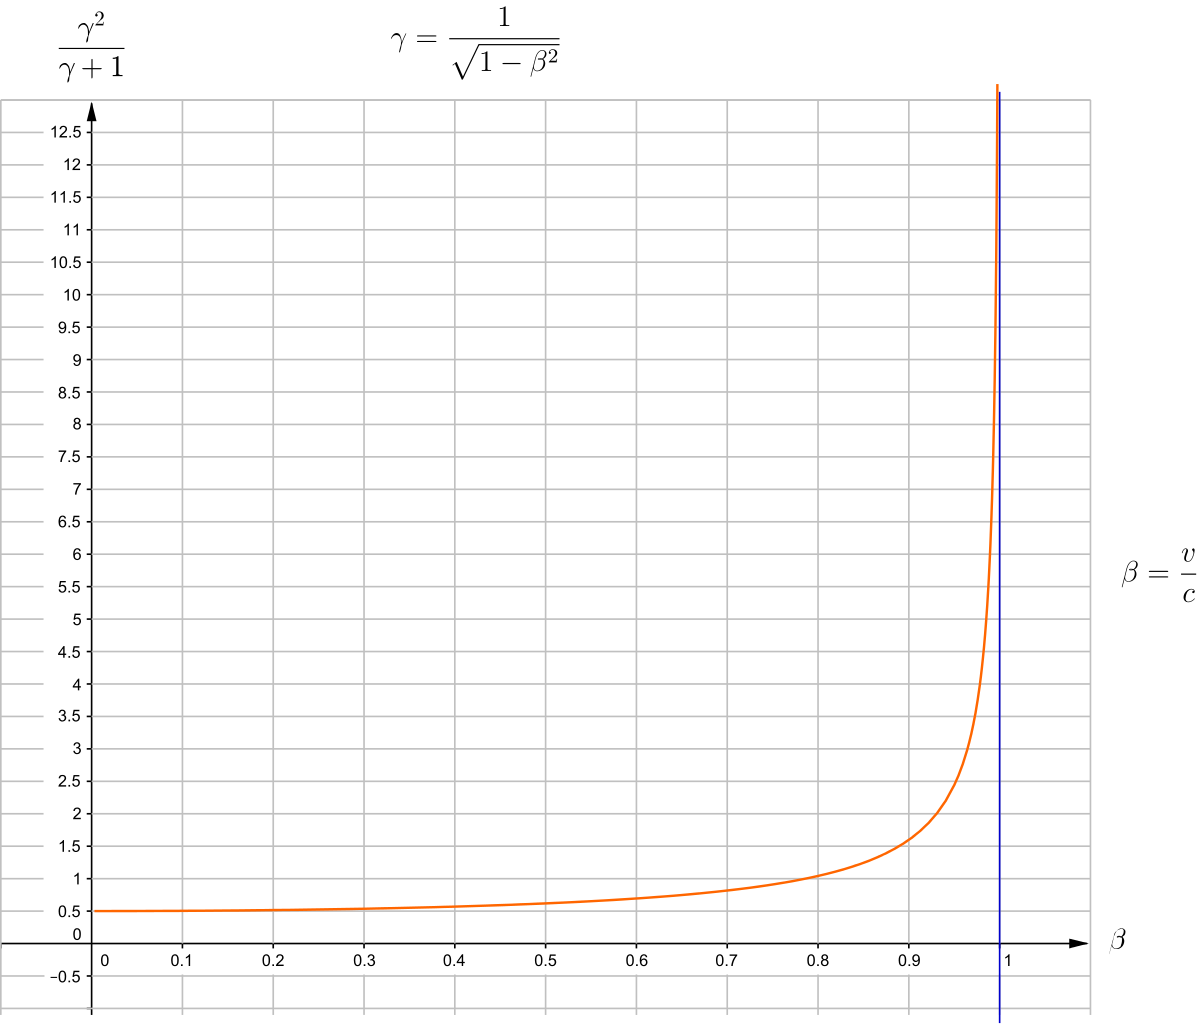
\includegraphics[width=8.5cm]{src/ThomasPrecession.png}}
        \scriptsize\CJKfamily{hwht}$\gamma^2/\pare{\gamma+1}$的值随$\beta = v/c$的变化情况, $v$是质点的瞬时速度. Thomas旋进在$\beta<0.5$时都是可以忽略的, 而在$0.5<\beta<0.8$时稳定增长, 接着随着$\beta$趋于$1$而迅速上升至无穷. Thomas减半因子在低速极限下可见, 旋进仅在接近光速时变得明显.
    \end{tcolorbox}
\end{wrapfigure}

考虑质点的运动. 引入实验室参考系$\Sigma$, 使得其中的观察者可以测量质点相对该参考系的运动. 每一个瞬间这个质点都有与之关联的惯性参考系, 使得该质点在其中静止. 相对于该实验室参考系, 质点的瞬时速度$\+vv\pare{t}$不能超过光速, $\abs{\+vv} = v < c$. 这里的$t$是实验室参考系中测得的时间, 并非质点的\href{https://en.wikipedia.org/wiki/Proper_time}{固有时}.
\par
除了受光速的约束外, 质点的速度是任意的且不一定为常数. 相应的加速度为$\displaystyle \+va = \+dtd{\+vv\pare{t}}$. 作为各瞬时的Wigner旋转的结果, 质点参考系以如下的速度旋进:
\begin{resume}
    \centerline{\textsf{Thomas}\CJKfamily{hwht}旋进}
    \[ \+v\omega\+_T_ = \rec{c^2}\pare{\frac{\gamma^2}{\gamma+1}}\+va\times \+vv, \]
\end{resume}
其中$\times$表示叉乘而
\[ \gamma = \rec{\sqrt{\displaystyle 1- \frac{\abs{\+vv\pare{t}}^2}{c^2}}} \]
是瞬时Lorentz因子, 作为质点瞬时速度的函数. 如同其它任何角速度, $\+v\omega\+_T_$是一个\href{https://en.wikipedia.org/wiki/Pseudovector}{赝矢量}, 其大小为质点参考系进动的速度(弧度每秒), 其方向指向旋转的方向. 如同往常, 此处叉乘采用右手定则.
\par
该旋进取决于\emph{加速运动}, 以及质点的瞬时速度和加速度的非共线性. 如果质点匀速运动($\+v$为常数而$\+va=0$)或者沿着直线加速(此时$\+vv$和$\+va$平行或反平行从而起叉乘为零), 旋进不会发生. 质点需要沿着曲线运动以发生旋进. 如果速度和加速度垂直则旋进角速度最大(圆周运动), 且速度和加速度的模长越大进动角速度越大(特别当$\+vv$接近$c$时).
\par
在非相对论情形下, $\+vv \rightarrow 0$故$\gamma \rightarrow 1$, 旋进角速度大约为
\[ \+v\omega\+_T_ = \rec{2c^2}\+va\times \+vv. \]
前面的$1/2$因子是理论预言和实验相符的关键因子, 通常称为Thomas减半因子.

% subsection 表达式 (end)

% section 导引 (end)

\section{数学推导} % (fold)
\label{sec:数学推导}

\subsection{Lorentz变换} % (fold)
\label{sub:lorentz变换}

对相对运动的完整描述需要使用Lorentz变换, 而其矩阵形式将会使计算更加简便. 以符号表示矩阵可以简洁地写出变换, 而当需要具体的矩阵分量时各分量也会被写出. 为了防止公式中出现过多的$c$, 这里引入定义$\+v\beta\pare{t} = \+vv\pare{t}/c$, 其模长为$\abs{\+v\beta} = \beta$, 且$0\le \beta < 1$.
\par
实验室参考系的时空坐标可以写入一个$4\times 1$的列向量, 而boost可以被表示为一$4\times 4$的对称矩阵.
\[ X = \begin{pmatrix}
    ct\\ x\\ y\\ z
\end{pmatrix},\quad B\pare{\+v\beta} = \begin{pmatrix}
    \displaystyle \gamma & -\gamma\beta_x & -\gamma\beta_y & -\gamma\beta_z \\
    \displaystyle -\gamma\beta_x & \displaystyle 1+\pare{\gamma - 1}\frac{\beta_x^2}{\beta^2} & \displaystyle \pare{\gamma-1}\frac{\beta_x \beta_y}{\beta^2} &\displaystyle  \pare{\gamma - 1}\frac{\beta_x \beta_z}{\beta^2} \\
    \displaystyle -\gamma\beta_y & \displaystyle \pare{\gamma - 1}\frac{\beta_y\beta_x}{\beta^2} & \displaystyle 1+\pare{\gamma-1}\frac{\beta_y^2}{\beta^2} & \displaystyle \pare{\gamma - 1}\frac{\beta_y \beta_z}{\beta^2} \\
    \displaystyle -\gamma\beta_z & \displaystyle \pare{\gamma - 1}\frac{\beta_z\beta_x}{\beta^2} &\displaystyle  \pare{\gamma-1}\frac{\beta_z \beta_y}{\beta^2} &\displaystyle  1+\pare{\gamma - 1}\frac{\beta_z^2}{\beta^2} \\
\end{pmatrix}. \]
其中
\[ \gamma = \rec{\sqrt{1-\abs{\+v\beta}^2}} \]
是$\+v\beta$的Lorentz因子. 在其它参考系中, 各坐标同样可以放入一列矢量中. Boost的逆矩阵为反方向的Boost, 由$B\pare{\+v\beta}^{-1} = B\pare{-\+v\beta}$给出.
\par
对于每个在实验室参考系中测的的时刻$t$, 从实验室参考系$\Sigma$到质点参考系$\Sigma'$的变换为
\begin{equation}
    \label{eq:第一boost}
    X' = B\pare{\+v\beta}X.
\end{equation}
在一小段时间后的实验室时刻$t+\Delta t$, 质点有新的参考系$\Sigma''$, 其以$\+v\beta + \Delta \+v\beta$相对$\Sigma$运动, 相应的boost为
\begin{equation}
    \label{eq:第二boost}
    X'' = B\pare{\+v\beta + \Delta \+v\beta} X.
\end{equation}
$\+v\beta$和$\Delta \+v\beta$是两个不同的向量. 后者是小增量, 可以分为相对于$\+v\beta$平行和垂直的部分,
\[ \Delta \+v\beta = \Delta \+v\beta_\parallel + \Delta \+v\beta_\perp. \]
结合\eqref{eq:第一boost}和\eqref{eq:第二boost}可得$\Sigma'$和$\Sigma''$间的Lorentz变换,
\begin{equation}
    \label{eq:结合boost}
    X'' = B\pare{\+v\beta + \Delta \+v\beta}B\pare{-\+v\beta}X',
\end{equation}
这一结合包含了两个实验室时刻间的运动的全部信息. 注意到$B\pare{\+v\beta + \Delta \+v\beta}B\pare{-\+v\beta}$和$B\pare{\+v\beta + \Delta \+v\beta}$是无限小变换, 因为其仅涉及相对速度的小增量, 而$B\pare{-\+v\beta}$则非无限小变换.
\par
两个boost的结合可以变为一个boost与一个绕与速度垂直轴的Wigner旋转的复合,
\begin{equation}
    \label{eq:复合boost}
    \Lambda = B\pare{\+v\beta + \Delta \+v\beta}B\pare{-\+v\beta} = R\pare{\Delta \+v\theta}B\pare{\Delta \+vb}.
\end{equation}
这一旋转由\href{https://en.wikipedia.org/wiki/Axis%E2%80%93angle_representation}{轴-角度表示}的旋转矩阵给出, 坐标系取右手系. 旋转矩阵将三维矢量顺时针绕轴转动, 亦即将参考系绕该轴逆时针旋转. 轴-角度矢量$\Delta \+v\theta$表征这一旋转, 其大小为$\Sigma''$转过的角度, 方向与转动轴平行, 此处平行于叉乘$\pare{-\+v\beta}\times \pare{\+v\beta + \Delta \+v\beta} = -\+v\beta\times\Delta\+v\beta$. 如果角度是负数, 则上面的定义应相应地调转. 其逆矩阵由$R\pare{\Delta \+v\theta}^{-1} = R\pare{-\Delta \+v\theta}$给出.
\par
与boost相关联的是一(小增量)boost向量$\Delta \+vb$, 其大小和方程是该boost的相对速度(除以$c$). $B\pare{\Delta \+vb}$这一boost和旋转变换$R\pare{\Delta \+v\theta}$都是无限小变换, 因为$\Delta \+vb$和$\Delta \+v\theta$是小量.
\par
这一旋转矩阵可以给出Thomas旋进, 但仍有一需要注意之处. 为了能将质点的参考系视为随其移动的相对实验室参考系为惯性参考系者, 且与非相对论性情形相符, 我们期望质点在$t$时刻和$t+\Delta t$时刻的瞬时参考系可以通过一不带旋转的boost相联系. 结合\eqref{eq:结合boost}和\eqref{eq:复合boost}可得
\begin{equation}
    \label{eq:第三boost}
    B\pare{\Delta \+vb} X' = R\pare{-\Delta \+v\theta}X'' = X'''.
\end{equation}
其中一个新的参考系$\Sigma'''$和相应的坐标$X'''$为了防止与$\Sigma''$冲突而被引入. 此处小结一下现存的参考系: 在实验室参考系$\Sigma$中观测着可以测量质点的运动, 而三个瞬时惯性参考系中质点在其中瞬间静止, $\Sigma'$对应时刻$t$, $\Sigma''$对应时刻$t+\Delta t$, $\Sigma'''$对应时刻$t+\Delta t$. 参考系$\Sigma''$和$\Sigma'''$的位置与时钟重合, 差别仅为一旋转. 而$\Sigma'$和$\Sigma'''$之间相差一个boost和以及实验室时间间隔$\Delta t$.
\par
通过\eqref{eq:第三boost}和\eqref{eq:第二boost}可以写出$X'''$和$X$之间的关系,
\[ X''' = R\pare{-\Delta \+v\theta}X'' = R\pare{-\Delta \+v\theta}B\pare{\+v\beta + \Delta \+v\beta} X. \]
其中$X'''$被反向旋转了.
\par
这一旋转是在两个不同的实验室时刻之间发生的. 当$\Delta\rightarrow 0$, 质点参考系的旋转各个时刻皆发生, 故质点的连续运动导致了以某个(可变)角速度的连续的旋转. 将$-\Delta \+v\theta$除以$\Delta t$, 并取$\Delta t \rightarrow 0$的极限, 可得角速度
\begin{equation}
    \label{eq:极限boost}
    \+v\omega\+_T_ = -\lim_{t\rightarrow 0} \frac{\Delta \+v\theta}{\Delta t}.
\end{equation}
剩下的就是找到$\Delta \+v\theta$的具体表达式.

% subsection lorentz变换 (end)

\subsection{提取结果} % (fold)
\label{sub:提取结果}

复合的记过可以由矩阵乘积展开得到. 为了得到$\+v\beta + \Delta \+v\beta$的boost, 需要知道这一向量的Lorentz因子. 由于$\Delta \+v\beta$是小量, 二阶量$\abs{\Delta \+v\beta}^2$, $\pare{\Delta \beta_x}^2$, $\pare{\Delta\beta_y}^2$, $\Delta\beta_x \Delta \beta_y$以及更高阶的项可以忽略. 考虑这一点后, 其模长为
\[ \abs{\+v\beta + \Delta \+v\beta}^2 = \abs{\+v\beta}^2 + 2\+v\beta\cdot \Delta \+v\beta. \]
将Lorentz因子展开为Taylor级数并提出$\Delta \+v\beta$的一阶项, 有
\begin{align*}
    & \rec{\sqrt{1-\abs{\+v\beta + \Delta \+v\beta}^2}} = 1+\half \abs{\+v\beta + \Delta \+v\beta}^2 + \frac{3}{8}\abs{\+v\beta + \Delta \+v\beta}^4 + \cdots \\
    &= \pare{1+\frac{\abs{\+v\beta}^2}{2} + \frac{3}{8}\abs{\+v\beta}^4 + \cdots} + \pare{1+\frac{3}{2}\abs{\+v\beta}^2 + \cdots}\+v\beta \cdot \Delta \+v\beta \\
    &\approx \gamma + \gamma^3 \+v\beta \cdot \Delta \+v\beta.
\end{align*}
其中$\+v\beta$的Lorentz因子$\gamma$定义如前文.
\par
引入boost生成元
\[ K_x = \begin{pmatrix}
    0 & 1 & 0 & 0 \\
    1 & 0 & 0 & 0 \\
    0 & 0 & 0 & 0 \\
    0 & 0 & 0 & 0
\end{pmatrix},\quad K_y = \begin{pmatrix}
    0 & 0 & 1 & 0 \\
    0 & 0 & 0 & 0 \\
    1 & 0 & 0 & 0 \\
    0 & 0 & 0 & 0
\end{pmatrix},\quad K_z = \begin{pmatrix}
    0 & 0 & 0 & 1 \\
    0 & 0 & 0 & 0 \\
    0 & 0 & 0 & 0 \\
    1 & 0 & 0 & 0
\end{pmatrix}, \]
以及旋转生成元
\[ J_x = \begin{pmatrix}
    0 & 0 & 0 & 0 \\
    0 & 0 & 0 & 0 \\
    0 & 0 & 0 & -1 \\
    0 & 0 & 1 & 0
\end{pmatrix},\quad J_y = \begin{pmatrix}
    0 & 0 & 0 & 0 \\
    0 & 0 & 0 & 1 \\
    0 & 0 & 0 & 0 \\
    0 & -1 & 0 & 0
\end{pmatrix},\quad J_z = \begin{pmatrix}
    0 & 0 & 0 & 0 \\
    0 & 0 & -1 & 0 \\
    0 & 1 & 0 & 0 \\
    0 & 0 & 0 & 0
\end{pmatrix}, \]
加上标量积$\cdot$即可得到坐标无关的表达式
\[ \Lambda = I - \pare{\frac{\gamma - 1}{\beta^2}}\pare{\+v\beta\times \Delta \+v\beta}\cdot \+vJ - \gamma\pare{\gamma\Delta \+v\beta_\parallel + \Delta \+v\beta_\perp}\cdot \+vK. \]
这一表达式对于任意平面内的$\+v\beta$和$\Delta \+v\beta$都成立. 这是boost和旋转组合成的无限小Lorentz变换,
\[ \Lambda = I - \Delta \+v\theta\cdot \+vJ - \Delta \+vb\cdot \+vK, \]
其中
\begin{align*}
    & \Delta \+v\theta = \pare{\frac{\gamma-1}{\beta^2}}\+v\beta\times \Delta \+v\beta = \rec{c^2}\pare{\frac{c^2}{\gamma+1}}\+vv\times \Delta \+vv,\\
    & \Delta \+vb = \gamma\pare{\gamma\Delta \+v\beta_\parallel + \Delta \+v\beta_\perp}.
\end{align*}
如\eqref{eq:极限boost}, 将$\Delta \+v\theta$除以$\Delta t$并取极限后
\[ \+v\omega\+_T_ = \rec{c^2}\pare{\frac{\gamma^2}{\gamma+1}}\+va\times \+vv. \]
其中$\+va$是实验室参考系中观测到的质点的加速度. 导出上述结果的过程与力的具体形式无关, 这是一个纯粹的几何效应. 然而, 是力导致了加速度, 因此Thomas旋进只有在对象受力的情况下才能被观察到.
\par
Thomas旋进也可以通过Fermi-Walker变换方程导出. 假设物体在平直的Minkowski空间内做匀速圆周运动, 自旋四维矢量垂直于速度四维矢量, 则Fermi-Walker变换保持这一性质. 可以证明加速度四维矢量和自旋四维矢量随时间以较频率$\gamma \omega$正弦变化, 其中$\omega$是运动的角频率而$\displaystyle \gamma = \rec{\sqrt{\displaystyle 1-\frac{v^2}{c^2}}}$. 这可以直接在点积中求二阶导数得到. 这一角频率超过$\omega$, 因此旋进发生在退行方向. 角频率的差$\pare{\gamma-1}\omega$正是Thomas旋进的角频率, 只需注意到三维加速度矢量的模长为$\omega v$.

% subsection 提取结果 (end)

% section 数学推导 (end)

\section{应用} % (fold)
\label{sec:应用}

\subsection{电子轨道} % (fold)
\label{sub:电子轨道}

量子力学中, \gloss{Thomas旋进}会向\href{https://en.wikipedia.org/wiki/Spin-orbit_interaction}{自旋-轨道作用}引入一修正, 这将氢原子中电子和原子核之间的钟慢效应纳入考虑.
\par
一言以蔽之, 自旋的加速物体会进动的原因在于Lorentz boost不是可交换的.
\par
为了得到磁场中粒子的正确自旋, 必须同时将Larmor进动纳入考虑.

% subsection 电子轨道 (end)

\subsection{Foucault摆} % (fold)
\label{sub:foucault摆}

Foucault摆的摆动平面的旋转可以视为在Euclid空间中的二维球面上平行移动摆的结果. Minkowski时空中的双曲速度空间是一具有虚半径和虚类时坐标的三维伪球面. 以相对论性速度平行移动具有自旋的粒子会引发Thomas旋进, 这和Foucault摆的转动有相似之处. 两者的转动角度都可以通过曲率的面积分确定, 与\href{https://en.wikipedia.org/wiki/Gauss%E2%80%93Bonnet_theorem}{Gau\ss-Bonnet定理}的结果一致.
\par
Thomas进动将对Foucault摆的进动引入一修正. 对于在荷兰Nijmegen市的Foucault摆, 相应的修正为
\[ \omega \approx \SI{9.5e-7}{\arcsecond\per\day}. \]
这比\href{https://en.wikipedia.org/wiki/Frame-dragging}{参考系拖拽}广义相对论性修正\href{https://en.wikipedia.org/wiki/Lense%E2%80%93Thirring_precession}{Lense-Thirring进动}小至少两个数量级.

% subsection foucault摆 (end)

% section 应用 (end)

\section{对原子能级的影响} % (fold)
\label{sec:对原子能级的影响}

这一节将给出对类氢原子中电子的自旋-轨道耦合相对简单的定量描述. 下面将采用半经典电动力学以及非相对论性量子力学的一阶近似, 可以得到与观测值足够吻合的结果.
\par
严格的计算需要采用\href{https://en.wikipedia.org/wiki/Relativistic_quantum_mechanics}{相对论性量子力学}和\href{https://en.wikipedia.org/wiki/Dirac_equation}{Dirac方程}, 并且将涉及多体相互作用. 为了得到更精确的结果需要考虑\href{https://en.wikipedia.org/wiki/Quantum_electrodynamics}{量子电动力学}引入的小修正.

\subsection{磁矩的能量} % (fold)
\label{sub:磁矩的能量}

磁矩在磁场中的能量由
\[ \Delta H = -\+v\mu\cdot \+vB \]
给出, 其中$\+v\mu$是磁矩, 而$\+vB$是它受到的磁场.

% subsection 磁矩的能量 (end)

\subsection{磁场} % (fold)
\label{sub:磁场}

我们现处理磁场. 虽然在原子核静止的参考系中没有磁场作用在电子上, 在电子静止的参考系中(参见\href{https://en.wikipedia.org/wiki/Classical_electromagnetism_and_special_relativity}{经典电磁学与狭义相对论})却存在这样的磁场. 忽略这一参考系并非惯性参考系之事实, 在SI单位制下有
\[ \+vB = -\frac{\+vv\times \+vE}{c^2}, \]
其中$\+vv$是电子的速度而$\+vE$为其所在处电场. 在非相对论极限下可以假设$\gamma \approx 1$. 由于$E$是径向的, $\+vE = \abs{E/r}\+vr$. 此外电子具有动量$\+vp = m\+_e_\+vv$, 代入可得
\[ \+vB = \frac{\+vr\times \+vp}{m\+_e_c^2}\abs{\frac{E}{r}}. \]
将电场用电势表示, $\+vE = -\grad V$, 此处采用中心场近似, 即静电势具有球对称性从而仅为径向距离之函数. 这一近似对于氢原子和类氢原子严格成立. 现在有
\[ \abs{E} = \+DrDV = \rec{e}\+DrD{U\pare{r}}, \]
其中$U = eV$是电子在中心场中的是能, $e$是基本电荷. 考虑到经典力学中的角动量为$\+vL = \+vr\times \+vp$, 代入得
\[ \+vB = \rec{m\+_e_ec^2} \rec{r} \+DrD{U\pare{r}} \+vL. \]
注意到$\+vB$是$\+vL$的某一正数倍, 从而磁场平行于电子的轨道角动量, 垂直于电子的速度.

% subsection 磁场 (end)

\subsection{电子的自旋磁矩} % (fold)
\label{sub:电子的自旋磁矩}

电子的\href{https://en.wikipedia.org/wiki/Spin_magnetic_moment}{自旋磁矩}为
\[ \+v\mu\+_S_ = -g\+_S_ \mu\+_B_ \frac{\+vS}{\hbar}. \]
其中$\+vS$是自旋角动量矢量, $\mu\+_B_$是\href{https://en.wikipedia.org/wiki/Bohr_magneton}{Bohr磁矩}, $g\+_S_ \approx 2$是电子自旋的\href{https://en.wikipedia.org/wiki/G-factor_(physics)}{$g$-因子}. 这里$\+v\mu$是自旋的负数倍, 故自旋磁矩和自旋角动量反平行.
\par
自旋-轨道相互作用由两部分组成. Larmor部分由电子自旋磁矩和原子核的相对运动产生的磁场之相互作用产生. 第二个贡献来源于Thomas旋进.

% subsection 电子的自旋磁矩 (end)

\subsection{Larmor相互作用能} % (fold)
\label{sub:larmor相互作用能}

Larmor相互作用能为
\[ \Delta H\+_L_ = -\+v\mu\cdot \+vB. \]
代入自旋磁矩和磁场的表达式, 可得
\[ \Delta H\+_L_ = \frac{2\mu_B}{\hbar m\+_e_ec^2} \rec{r} \+DrD{U\pare{r}} \+vL\cdot \+vS. \]
现在需要考虑电子的曲线轨道导致的Thomas旋进带来的修正.

% subsection larmor相互作用能 (end)

\subsection{Thomas相互作用能} % (fold)
\label{sub:thomas相互作用能}

1926年Llewellyn Thomas考虑了相对论效应后重新计算了氢原子的精细结构双线的间隔. Thomas进动速率$\+v\Omega\+_T_$和轨道运动频率$\+v\omega$之间的关系为
\[ \+v\Omega\+_T_ = \+v\omega\pare{\gamma - 1}. \]
其中$\gamma$是运动粒子的Lorentz因子. 生成这一进动速率的Hamiltonian为
\[ \Delta H\+_T_ = \+v\Omega\+_T_ \cdot \+vS. \]
在一阶近似下有
\[ \Delta H\+_T_ = -\frac{\mu\+_B_}{\hbar m_e ec^2}\rec{r}\+DrD{U\pare{r}}\+vL\cdot \+vS. \]

% subsection thomas相互作用能 (end)

\subsection{总相互作用能} % (fold)
\label{sub:总相互作用能}

外电磁势中总的自旋-轨道势能为
\[ \Delta H = \Delta H\+_L_ + \Delta H\+_T_ = \frac{\mu\+_B_}{\hbar m\+_e_ec^2}\rec{r}\+DrD{U\pare{r}}\+vL\cdot \+vS. \]
Thomas旋进的净作用即将Larmor相互作用能减少$1/2$, 故谓之Thomas减半因子.

% subsection 总相互作用能 (end)

\subsection{能级移动} % (fold)
\label{sub:能级移动}

通过上面的近似, 现在可以准确地计算这一模型下的能级移动. 注意到$L_z$和$S_z$此时不再是守恒量. 特别地, 我们希望能够找到一组新的基使得$H_0$和$\Delta H$同时对角化. 为了找到这组基, 定义\href{https://en.wikipedia.org/wiki/Azimuthal_quantum_number#Total_angular_momentum_of_an_electron_in_the_atom}{总角动量算符}
\[ \+vJ = \+vL + \+vS. \]
自点乘得
\[ \+vJ^2 = \+vL^2 + \+vS^2 + 2\+vL\cdot \+vS, \]
(注意到$\+vL$和$\+vS$是交换的). 从而
\[ \+vL\cdot \+vS = \half \pare{\+vJ^2 - \+vL^2 - \+vS^2}. \]
可以证明$H_0$, $\+vJ^2$, $\+vL^2$, $\+vS^2$和$J_z$彼此可交换, 且阶与$\Delta H$可交换. 故所寻找的基正是将这五个算符同时对角化者. 这一基的元素有五个量子数, 主量子数$n$, 总角量子数$j$, 总轨道角量子数$l$, 自旋量子数$s$, 总角动量磁量子数$j_z$.
\par
为了计算总能量, 注意到对于氢原子有
\[ \expc{\rec{r^3}} = \frac{2}{a^3n^3 l\pare{l+1}\pare{2l+1}}, \]
其中$a = \hbar/\pare{Z\alpha m_e c}$是\href{https://en.wikipedia.org/wiki/Bohr_radius}{Bohr半径}除以$Z$, 而
\[ \expc{\+vL\cdot \+vS} = \half\pare{\expc{\+vJ^2} - \expc{\+vL^2} - \expc{\+vS^2}} = \frac{\hbar^2}{2}\brac{j\pare{j+1} - l\pare{l+1} - s\pare{s+1}}. \]

% subsection 能级移动 (end)

\subsection{最终能级移动} % (fold)
\label{sub:最终能级移动}

现在有
\[ \resumath{\Delta E = \frac{\beta}{2}\pare{j\pare{j+1} - l\pare{l+1} - s\pare{s+1}}.} \]
其中
\[ \beta = \beta\pare{n,l} = Z^4 \frac{\mu_0}{4\pi}g_s \mu_B^2 \rec{n^3 a_0^3 l\pare{l+1/2}\pare{l+1}}. \]
关于精确的相对论解, 参阅\href{https://en.wikipedia.org/wiki/Hydrogen-like_atom#Solution_to_Dirac_equation}{类氢原子系统的Dirac方程的解.}

% subsection 最终能级移动 (end)

% section 对原子能级的影响 (end)

\section{参阅} % (fold)
\label{sec:参阅}

\begin{citem}
    \item \href{https://en.wikipedia.org/wiki/Velocity-addition_formula}{速度加法公式}
    \item \href{https://en.wikipedia.org/wiki/Relativistic_angular_momentum}{相对论性角动量}
\end{citem}

% section 参阅 (end)

\end{document}
